\newpage
%\thispagestyle{empty}
\begin{recipe}[source={Propia},
portion={4-5 porciones},
preparationtime={\unit[4]{h}\unit[15]{m}}
]{Carne Mechada}
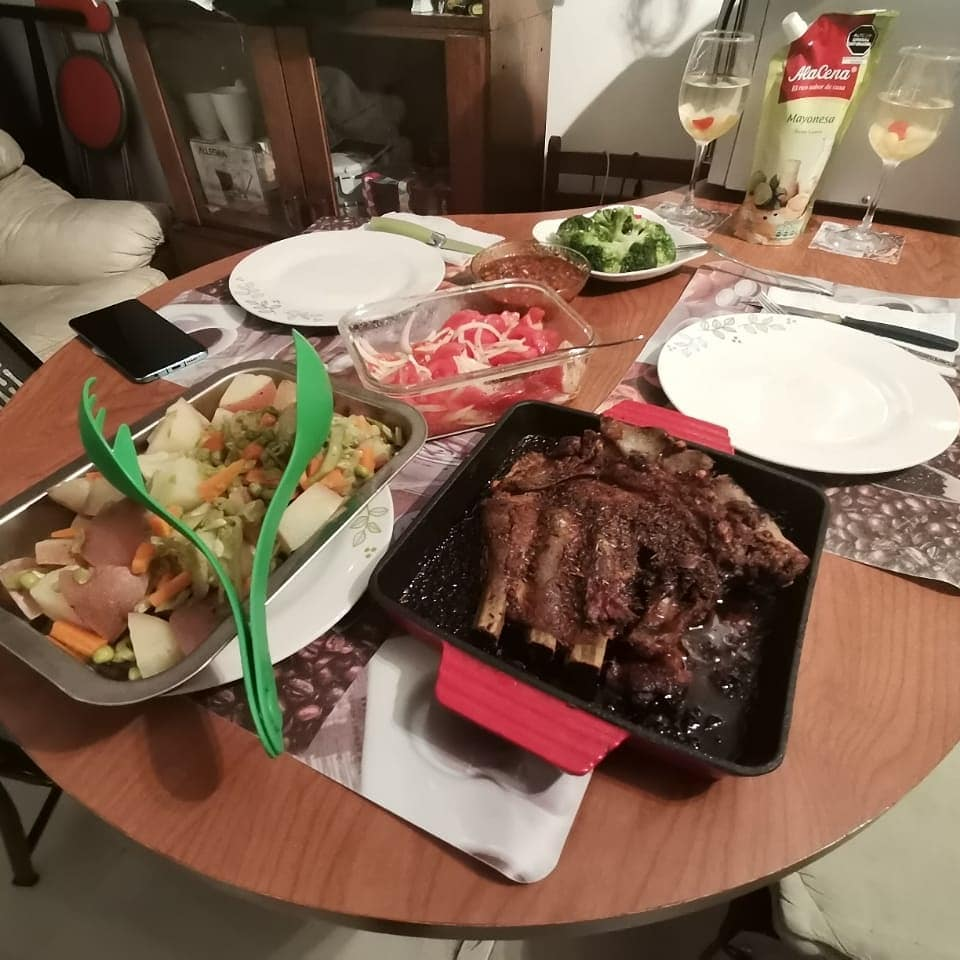
\includegraphics[width=0.25\textwidth]{costillar}
\introduction{
Esta es una receta propia.
}
\ingredients{
    1 & apio \\
    1 & cabeza de ajo \\
    6 & bastoncitos de zanahoria \\
    2 & tomates grandes y maduros \\
    1/2 & taza de apio para la salsa \\
    2 & cucharaditas de orégano \\
    2 & cucharaditas de ají de color \\
    & Sal a gusto \\
    & Pimienta molida a gusto \\
    & Comino a gusto \\
    & Orégano a gusto \\
    & Paprika o pimentón dulce a gusto \\
    1 & cucharada de aceite de oliva
}
\preparation{
    \begin{enumerate}
        \item Enbardunar las costillas con los aliños y dejar macerar.
        \item Tapar con film de aluminio y meter al horno pre calentado.
        \item Cocinar por una hora al horno. 
        \item Transcurrida la hora, apagar el horno y dejar enfriar en el mismo horno por 3 horas más.
        \item Quitar papel de aluminio.
        \item Pincelar con la salsa y calentar otra vez por 15 min.
    \end{enumerate}
}
\end{recipe}